\documentclass{article}
\usepackage[margin = 0.5in]{geometry}
\usepackage{amsfonts, setspace, graphicx, amsmath, bbm, enumerate}
\graphicspath{{./images/}}

\begin{document}
    \onehalfspacing

    \begin{singlespace}
        \title{CSE 417T: Homework 4} 
        \author{Hangxiao Zhu}
        \date{\today}
        \maketitle
    \end{singlespace}

    \section*{Problem 1.}
    a. Plot the OOB error for bagging decision trees with the number of bags from 1 to 200:
    \begin{figure}[!htb]
        \begin{center}
            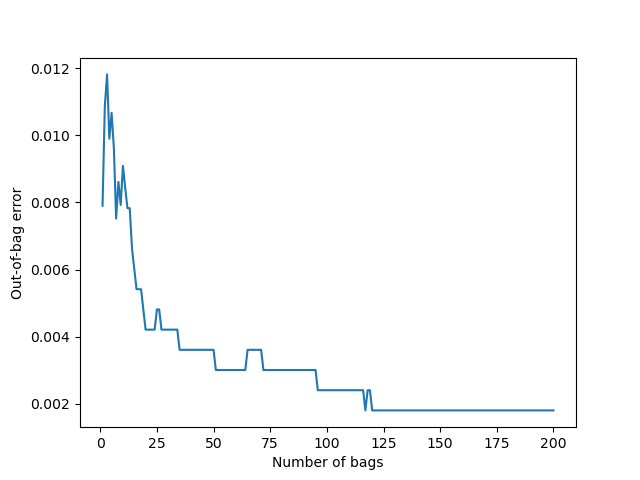
\includegraphics[width=10.24cm, height=7.68cm]{one_three.png}
            \textbf{\caption{OOB Error for ``1-vs-3'' Problem}}
        \end{center}
    \end{figure}
    \begin{figure}[!htb]
    \begin{center}
        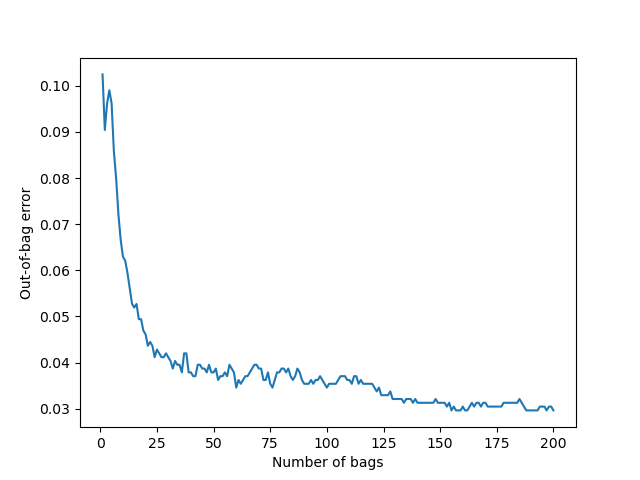
\includegraphics[width=10.24cm, height=7.68cm]{three_five.png}
        \textbf{\caption{OOB Error for ``3-vs-5'' Problem}}
    \end{center}
    \end{figure}\\
    b. Report the OOB error of bagging decision trees and the test errors of (1) a single decision tree 
    and (2) bagging decision trees:
    \begin{center}
        \begin{tabular}{|c|c|c|}
            \hline
            \multicolumn{3}{| c |}{\textbf{``1-vs-3'' Problem}}\\
            \hline
            & OOB error & Test error\\
            \hline
            Bagging Decision Trees & 0.0018039687312086591 & 0.011627906976744186\\
            \hline
            Single Decision Tree & N/A & 0.01627906976744186\\
            \hline
        \end{tabular}
    \end{center}
    \begin{center}
        \begin{tabular}{|c|c|c|}
            \hline
            \multicolumn{3}{| c |}{\textbf{``3-vs-5'' Problem}}\\
            \hline
            & OOB error & Test error\\
            \hline
            Bagging Decision Trees & 0.029654036243822075 & 0.07668711656441718\\
            \hline
            Single Decision Tree & N/A & 0.1196319018404908\\
            \hline
        \end{tabular}
    \end{center}
    c. Summary and Interpretation:
    \begin{itemize}
        \item Both Bagging Decision Trees and Single Decision Tree have better performance in the 
        1-vs-3 problem. That is, the OOB error and test error of the 1-vs-3 problem are 
        smaller than those of the 3-vs-5 problem. This may be because in the 1-vs-3 problem, 
        1 and 3 have more distinct characteristic differences, such as symmetries. But in 
        the 3-vs-5 problem, the difference in characteristics between 3 and 5.
        \item The OOB error can be significantly reduced by increasing the number of bags, because 
        when the number of bags is small, there are some points that appear in all the bootstrapped datasets.
        \item According to the experimental results, the OOB error and test error are very close to each 
        other. This makes sense since OOB error is an estimate of the error for unseen data, we can consider 
        the OOB error as an unbiased estimation of the test error.
    \end{itemize}

    \section*{Problem 2.}
    The formula to be used to solve this problem:
    \begin{align*}
        H(D) &= \sum_{i = 1}^{K} p_i \log_{2}\frac{1}{p_i}\\
        Gain(D, A) &= H(D) - \sum_{i} \frac{|D_i|}{|D|} H(D_i)
    \end{align*}
    The original Information Entropy of this dataset:
    \begin{align*}
        H(D) &= \frac{3}{5} \log_{2}\frac{5}{3} + \frac{2}{5} \log_{2}\frac{5}{2}\\
        &\approx 0.971
    \end{align*}
    a. To determine the root attribute of the tree, I will discuss three diferent cases:\\
    \textbf{Case 1.} With Color as root:
    \begin{align*}
        Gain(D, Color) &= H(D) - \sum_{i} \frac{|D_i|}{D_i} H(D_i)\\
        &= 0.971 - (\frac{|D_{Purple}|}{|D|} H(D_{Purple}) + \frac{|D_{Red}|}{|D|} H(D_{Red}))\\
        &= 0.971 - (\frac{4}{5} \times (\frac{1}{2} \log_{2}2 + \frac{1}{2} \log_{2}2) + 
        \frac{1}{5} \times \log_{2}1)\\
        &= 0.971 - (\frac{4}{5} \times 1 + \frac{1}{5} \times 0)\\
        &= 0.971 - 0.8\\
        &= 0.171
    \end{align*}
    \textbf{Case 2.} With Stripes as root:
    \begin{align*}
        Gain(D, Stripes) &= H(D) - \sum_{i} \frac{|D_i|}{D_i} H(D_i)\\
        &= 0.971 - (\frac{|D_{No}|}{|D|} H(D_{No}) + \frac{|D_{Yes}|}{|D|} H(D_{Yes}))\\
        &= 0.971 - (\frac{2}{5} \times \log_{2}1 + \frac{3}{5} \times 
        (\frac{1}{3} \log_{2}3 + \frac{2}{3} \log_{2}\frac{3}{2}))\\
        &\approx 0.971 - (\frac{2}{5} \times 0 + \frac{3}{5} \times 0.918)\\
        &= 0.971 - 0.5508\\
        &= 0.4202\\
        &\approx 0.420
    \end{align*}
    \textbf{Case 3.} With Texture as root:
    \begin{align*}
        Gain(D, Stripes) &= H(D) - \sum_{i} \frac{|D_i|}{D_i} H(D_i)\\
        &= 0.971 - (\frac{|D_{Smooth}|}{|D|} H(D_{Smooth}) + \frac{|D_{Rough}|}{|D|} H(D_{Rough}))\\
        &= 0.971 - (\frac{3}{5} \times (\frac{1}{3} \log_{2}3 + \frac{2}{3} \log_{2}\frac{3}{2}) + 
        \frac{2}{5} \times (\frac{1}{2} \log_{2}2 + \frac{1}{2} \log_{2}2))\\
        &\approx 0.971 - (\frac{3}{5} \times 0.918 + \frac{2}{5} \times 1)\\
        &= 0.971 - 0.9508\\
        &= 0.0202\\
        &\approx 0.020
    \end{align*}
    According to the above calculation results, we have $Gain(D, Stripes) > Gain(D, Color) > Gain(D, Stripes)$.
    Thus we should choose Stripes as the root attribute of the tree.
    \newpage
    b. The decision tree obtained using ID3:
    \begin{figure}[!htb]
        \begin{center}
            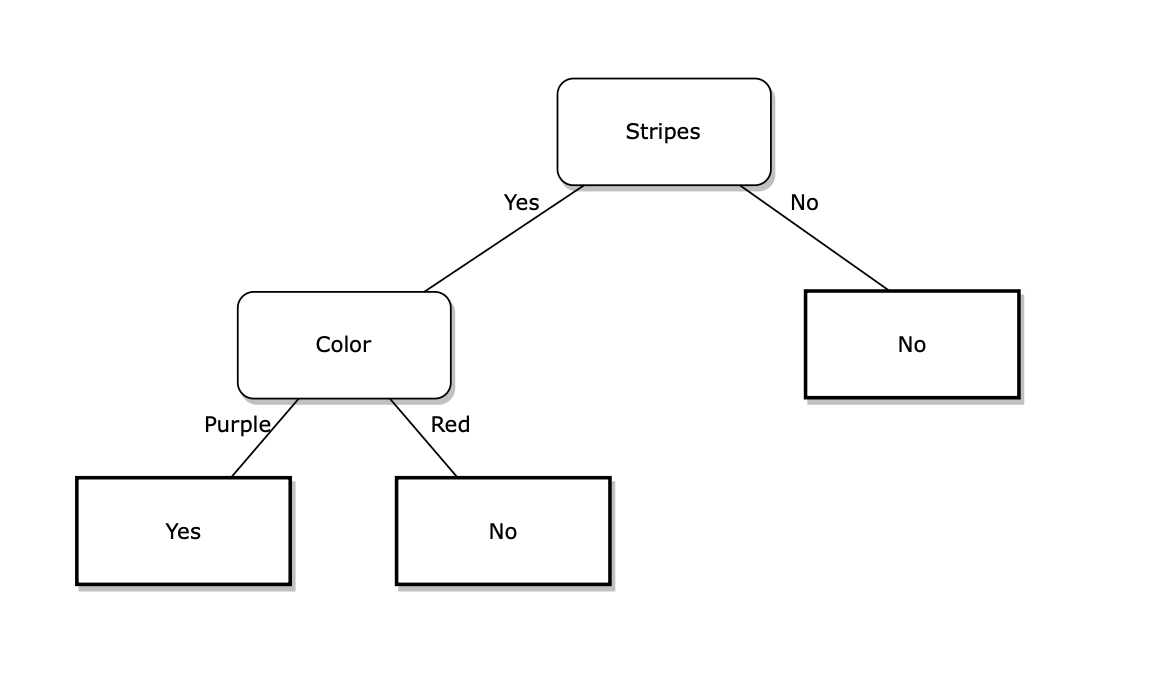
\includegraphics[width=11.72cm, height=6.82cm]{Q2.png}
        \end{center}
    \end{figure}

    \section*{Problem 3.}
    Since at the first iteration, 80\% of the data points were positive and 20\% of the data points were 
    negative, we can define $\epsilon_1 = 0.2$. Then we can define 
    \begin{align*}
        \alpha_1 &= \frac{1}{2}\ln(\frac{1 - \epsilon_1}{\epsilon_1}) = \frac{1}{2}\ln4
    \end{align*}
    Then we have 
    \begin{align*}
        e^{\alpha_1} &= \sqrt[2]{\frac{1 - \epsilon_1}{\epsilon_1}} = 2
    \end{align*} 
    Therefore the update rule for $D_2$ will be 
    \begin{align*}
        D_2(n) &= \frac{1}{Z_1} D_1(n) e^{-\alpha_1 g_1(\overset{\to}{x_n}) y_n}
    \end{align*}
    For positive points, 
    \begin{align*}
        D_2(n) &= \frac{1}{Z_1} D_1(n) e^{-\alpha_1}\\
        &= \frac{1}{Z_1} D_1(n) \times \frac{1}{2}\\
        &= \frac{1}{Z_1} \frac{D_1(n)}{2}
    \end{align*}
    Thus the cumulative weight of positive points is 
    \begin{align*}
        \sum \frac{1}{Z_1} \frac{D_1(n)}{2} &= \frac{1}{Z_1} \sum \frac{\frac{1}{N}}{2}\\
        &= \frac{1}{Z_1} \times 0.8N \times \frac{1}{2N}\\
        &= \frac{1}{Z_1} \times 0.4\\
    \end{align*}
    For negative points,
    \begin{align*}
        D_2(n) &= \frac{1}{Z_1} D_1(n) e^{\alpha_1}\\
        &= \frac{1}{Z_1} D_1(n) \times 2\\
        &= \frac{1}{Z_1} 2D_1(n)
    \end{align*}
    Thus the cumulative weight of negative points is 
    \begin{align*}
        \sum \frac{1}{Z_1} 2D_1(n) &= \frac{1}{Z_1} \sum 2 \times \frac{1}{N}\\
        &= \frac{1}{Z_1} \times 0.2N \times \frac{2}{N}\\
        &= \frac{1}{Z_1} \times 0.4\\
    \end{align*}
    After normalization, the cumulative weight of positive points is 0.5, the cumulative weight of negative
    points is 0.5.\\
    Based on this result, I don't think using depth 0 decision trees as weak learners is a good idea. Because 
    the the cumulative weight of positive points and negative points are equal to each other, which means we 
    did not achieve the goal of boosting and the aggregated leaner will not perform better. In the extreme case, 
    if the weights of each positive and negative points are identical, it may even result in that the model 
    perform the same as random guess.

    \section*{Problem 4.}
    First, bagging is theoretically suitable for a large number of weak learners with high variance and 
    low bias, while linear regression is a low variance learner. Second, we can imagine that when the point 
    correlation within our dataset is low, there is often no suitable linear model fit their characteristics.
    Therefore, after bagging, the linear regression models generated by each bag may vary greatly, that is,
    the weak learners will have high bias. The problem of high bias is difficult to be solved with the bagging 
    method, so the model will end up with poor performance. In addition, due to the random nature of sampling, 
    even data sets that originally have linear properties may show nonlinear characteristics in each bag, which
    could lead to decreased accuracy in the hyphthesis set and thus decreased accuracy in the final hypothesis.

    \section*{Problem 5.}
    a. Summary:\\
    I chose Topic 1: Facial recogition and read the article \textit{Study finds gender and skin-type bias in 
    commercial artificial-intelligence systems}. This article discusses the presence of skin type and gender 
    bias in commercially available facial analysis programs released by three major technology companies. 
    This probelm was revealed by Joy Buolamwini, a researcher in the MIT Media Lab's Civic Media 
    group, when she was working on a system called "Upbeat Walls" when she discovered that this system 
    could only be used reliably with lighter-skinned team members, which meant that the commercial facial 
    analysis program used by the system might be flawed. Buolamwini then collected over 1200 images that 
    better represent the characteristics of women and people with dark skin to test three commercially 
    available facial analysis programs. These systems all performed poorly, with error rates increasing as the 
    skin tones, according to the Fitzpatrick scale, of the people in the test images deepened. In particular, 
    when testing the darkest-skinned women in the dataset - those assigned VI scores - two of the systems even 
    reached error rates of 46.5\% and 46.8\%, which approximates to random guesses. Such test results indicate 
    that the training data for these models are heavily weighted towards males and light-skinned people. The 
    new benchmark proposed by Buolamwini's research are now reflected in a different and robust underlying 
    neural network designed for IBM's Watson artificial-intelligence system.\\
    b. Rephrase the issues:\\
    Based on what I have learned in this lesson, the issue raised in this article can be seen as a result 
    of sampling bias, i.e., If the data is sampled in a biased way, learning will produce a similarly biased 
    outcome. The commercially released facial-analysis programs mentioned in this article resulted in 
    invalid results because they did not ensure that the training and testing distributions were the same. For 
    example, according to the article, the dataset used to evaluate a face recognition system designed by a 
    large U.S. technology company was more than 77\% male and more than 83\% white, thus the performance of the 
    face recognition system evaluated based on this criterion was biased because this dataset attenuated 
    the effect of females and darker ethnicities.\\
    c. Potential approaches to mitigate the issues:
    \begin{itemize}
        \item Use broader training datasets which are highly balanced across skin phenotype and gender. This 
        eliminates the effect of sampling bias since the datasets evenly covers people of different skin color 
        and gender.
        \item Create test datasets covering each skin color class based on the Fitzpatrick score, and set the 
        same target for test errors for each skin color class's datasets. This avoids bias in the test results
        because if only a composite dataset is used for testing, the test results will not reflect whether there 
        are differences in the model's performance when dealing with data of different skin color and gender.
        \item Based on the assumption of VC analysis, the training dataset should be generated from the same 
        distribution of the test data set, thus the training datasets and the test datasets described above 
        should follow this rule. If the amount of data is not sufficient, we can apply Cross Validation to make 
        full use of the data we obtain.
    \end{itemize}

\end{document}